% ----- 04 — Leadership: NOLS model (full text from sample) -----

\section{Debriefing Guides and Frameworks}\label{sec:leadership}

\subsection{NOLS Leadership Model}

\subsubsection{The 4 NOLS Leadership Roles}

\begin{center}
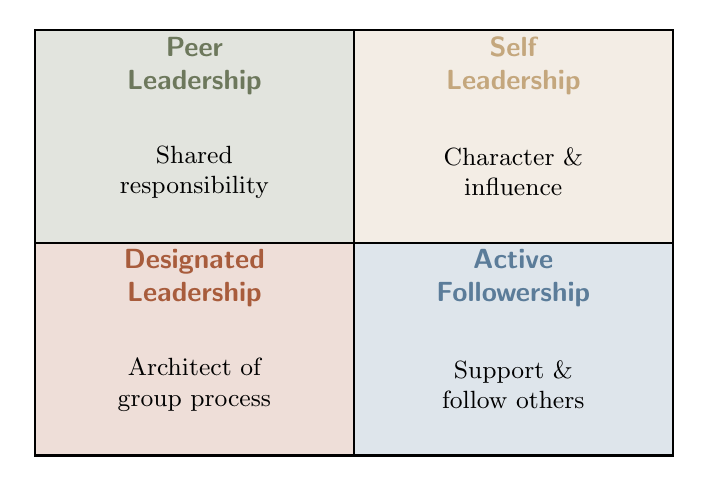
\begin{tikzpicture}[scale=0.9]
  % Define colors
  \definecolor{role1}{RGB}{168,92,60}
  \definecolor{role2}{RGB}{91,124,153}
  \definecolor{role3}{RGB}{109,120,92}
  \definecolor{role4}{RGB}{196,167,125}

  % Draw four quadrants
  \fill[role1!20] (0,0) rectangle (4.5,3);
  \fill[role2!20] (4.5,0) rectangle (9,3);
  \fill[role3!20] (0,3) rectangle (4.5,6);
  \fill[role4!20] (4.5,3) rectangle (9,6);

  % Add role labels
  \node[font=\sffamily\bfseries, color=role1, align=center] at (2.25,2.5) {Designated\\Leadership};
  \node[font=\sffamily\bfseries, color=role2, align=center] at (6.75,2.5) {Active\\Followership};
  \node[font=\sffamily\bfseries, color=role3, align=center] at (2.25,5.5) {Peer\\Leadership};
  \node[font=\sffamily\bfseries, color=role4, align=center] at (6.75,5.5) {Self\\Leadership};

  % Add brief descriptions
  \node[font=\small, align=center, text width=4cm] at (2.25,1) {Architect of\\group process};
  \node[font=\small, align=center, text width=4cm] at (6.75,1) {Support \&\\follow others};
  \node[font=\small, align=center, text width=4cm] at (2.25,4) {Shared\\responsibility};
  \node[font=\small, align=center, text width=4cm] at (6.75,4) {Character \&\\influence};

  % Draw borders
  \draw[thick] (0,0) rectangle (9,6);
  \draw[thick] (4.5,0) -- (4.5,6);
  \draw[thick] (0,3) -- (9,3);
\end{tikzpicture}
\end{center}

\vspace{0.5em}

\begin{enumerate}[noitemsep]
  \item \textbf{Designated Leadership:} Head architect and guardian of group process. Can delegate but not abdicate responsibility.

  \item \textbf{Active Followership:} Show leadership by following others. Seek clarity, give input, respect the plan, work for group betterment.

  \item \textbf{Peer Leadership:} Each person sees what needs to be done and does it without hierarchy. Works best with clear responsibilities.

  \item \textbf{Self-Leadership:} Lead through character and judgment, not position. Influence others through who you are.
\end{enumerate}

\subsubsection{The 7 NOLS Leadership Skills}

\begin{center}
\begin{tikzpicture}
  % Define colors
  \definecolor{skill}{RGB}{168,92,60}

  % Central circle
  \node[circle, draw=skill, fill=skill!10, minimum size=2cm, align=center, thick] (center) {\textbf{NOLS}\\Leadership};

  % Skills around the circle (7 skills)
  \foreach \angle/\skill in {90/Expedition Behavior, 141/Competence, 192/Communication, 243/Judgment, 294/Tolerance, 345/Self-Awareness, 39/Vision \& Action} {
    \node[circle, draw=skill, fill=atacamaCream, minimum size=1.2cm, align=center, font=\tiny\sffamily] at (\angle:3.5cm) {\skill};
    \draw[->, thick, skill] (center) -- (\angle:2.3cm);
  }
\end{tikzpicture}
\end{center}

\vspace{1em}

\textbf{1. Expedition Behavior:} Serve the group mission; treat everyone with dignity; support growth in others; do your share; model integrity; resolve conflict productively.

\textbf{2. Competence:} Build knowledge and skills continuously; set goals and follow through; maintain yourself as a high-functioning team member.

\textbf{3. Communication Skills:} Speak up when appropriate; set clear expectations; listen actively; use "I" language; give timely, growth-oriented feedback; stay open to receiving feedback.

\textbf{4. Judgment \& Decision-Making:} Develop situational awareness; choose appropriate decision-making styles and communicate them; leverage team strengths; help others see the big picture; question assumptions.

\textbf{5. Tolerance for Adversity \& Uncertainty:} Turn challenges into opportunities; see multiple workable options; embrace hard work; control what you can; use humor; stay connected under pressure; work with all personality types.

\textbf{6. Self-Awareness:} Know your abilities and limitations; learn from experience and mistakes; be authentic; communicate your values and goals; balance work, play, reflection, and rest; seek feedback.

\textbf{7. Vision \& Action:} Initiate what needs to be done; inspire others to reach their potential; balance empathy with decisiveness; align actions with group values; take appropriate risks; lead by example.

\vspace{2cm}

\clearpage
